% https://tex.stackexchange.com/questions/51757/how-can-i-use-tikz-to-make-standalone-svg-graphics
\documentclass{standalone}
\usepackage[svgnames]{xcolor} % Enabling colors by their 'svgnames'
\usepackage{tikz}
\usetikzlibrary{calc}
\usepackage{amsmath,amsfonts,amsthm}
\usepackage{physics}

\begin{document}
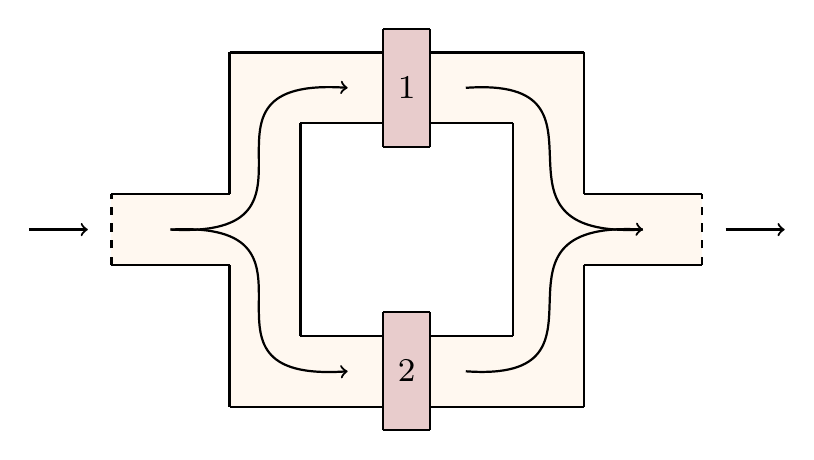
\begin{tikzpicture}[scale=1.5, every node/.style={scale=1.5}]
    
    %Ring coloring
    \fill[color=DarkOrange!6] (1,-1.5) rectangle (1.6,1.5); %Left
    \fill[color=DarkOrange!6] (1.6,0.9) rectangle (2.3,1.5); %Top left
    \fill[color=DarkOrange!6] (2.7,0.9) rectangle (3.4,1.5); %Top right
    \fill[color=DarkOrange!6] (3.4,-1.5) rectangle (4,1.5); %Right
    \fill[color=DarkOrange!6] (1.6,-0.9) rectangle (2.3,-1.5); %Lower left
    \fill[color=DarkOrange!6] (2.7,-0.9) rectangle (3.4,-1.5); %Lower right
    
    %Left input
    \fill[color=DarkOrange!6] (0,-0.3) rectangle (1,0.3); %Fill with color
    \draw[thick] (0,0.3) -- (1,0.3); %Top line
    \draw[thick] (0,-0.3) -- (1,-0.3); %Lower line
    \draw[thick, dashed] (0,-0.3) -- (0,0.3); %Left dashed line
        
    %Outer ring
    \draw[thick] (1,0.3) -- (1,1.5);     %Left outer up line
    \draw[thick] (1,-0.3) -- (1,-1.5);   %Left outer down line
    \draw[thick] (1,1.5) -- (2.3,1.5);   %Top left outer line
    \draw[thick] (2.7,1.5) -- (4,1.5);   %Top right outer line
    \draw[thick] (4,0.3) -- (4,1.5);     %Right outer up line
    \draw[thick] (4,-0.3) -- (4,-1.5);   %Right outer down line
    \draw[thick] (1,-1.5) -- (2.3,-1.5); %Lower left outer line
    \draw[thick] (2.7,-1.5) -- (4,-1.5); %Lower right outer line
    
    %Inner ring
    \draw[thick] (1.6,-0.9) -- (1.6,0.9); %left inner ring line
    \draw[thick] (1.6,0.9) -- (2.3,0.9);  %top inner ring line L
    \draw[thick] (2.7,0.9) -- (3.4,0.9);  %top inner ring line R
    \draw[thick] (3.4,0.9) -- (3.4,-0.9); %right inner ring line
    \draw[thick] (1.6,-0.9) -- (2.3,-0.9);%lower inner ring line L
    \draw[thick] (2.7,-0.9) -- (3.4,-0.9);%lower inner ring line R
    
    %Right output
    \fill[color=DarkOrange!6] (4,-0.3) rectangle (5,0.3); %Fill with color
    \draw[thick] (4,0.3) -- (5,0.3); %Top line
    \draw[thick] (4,-0.3) -- (5,-0.3); %Lower line
    \draw[thick, dashed] (5,-0.3) -- (5,0.3); %Left dashed line
    
    %Insulators
    %Top Insulator
    \fill[color=DarkRed!20] (2.3,0.7) rectangle (2.7,1.7); %Fill with color
    \draw[thick] (2.3,0.7) -- (2.3,1.7); %Left
    \draw[thick] (2.7,0.7) -- (2.7,1.7); %Right
    \draw[thick] (2.3,1.7) -- (2.7,1.7); %Top
    \draw[thick] (2.3,0.7) -- (2.7,0.7); %Lower
    %Bottom Insulator
    \fill[color=DarkRed!20] (2.3,-1.7) rectangle (2.7,-0.7); %Fill with color
    \draw[thick] (2.3,-1.7) -- (2.3,-0.7); %Left
    \draw[thick] (2.7,-1.7) -- (2.7,-0.7); %Right
    \draw[thick] (2.3,-0.7) -- (2.7,-0.7); %Top
    \draw[thick] (2.3,-1.7) -- (2.7,-1.7); %Lower
    
    %In-out arrows and text
    \draw[thick,->] (-0.7,0) -- (-0.2,0); % In arrow
    \draw[thick,->] (5.2,0) -- (5.7,0); % Out arrow
    
    % Current lines.
    \draw[thick,->] (0.5,0) .. controls (2,-0.08) and (0.5,1.3) .. (2,1.2); %Left up
    \draw[thick,->] (0.5,0) .. controls (2,0.08) and (0.5,-1.3) .. (2,-1.2);%Left down
    \draw[thick] (3,1.2) .. controls (4.4,1.3) and (3,-0.08) .. (4.5,0); %Right up
    \draw[thick,->] (3,-1.2) .. controls (4.4,-1.3) and (3,0.08) .. (4.5,0);%Right down
    
    %Insulator numbers.
    \node at (2.5,1.2) {\footnotesize 1}; %Up
    \node at (2.5,-1.2) {\footnotesize 2}; %Bottom
    
\end{tikzpicture}
\end{document}
